\fontsize{13px}{13px}\selectfont\justifying

\subsection{Sơ đồ thành phần}

\begin{figure}[h!]\fontsize{13px}{13px}\selectfont
\centering
		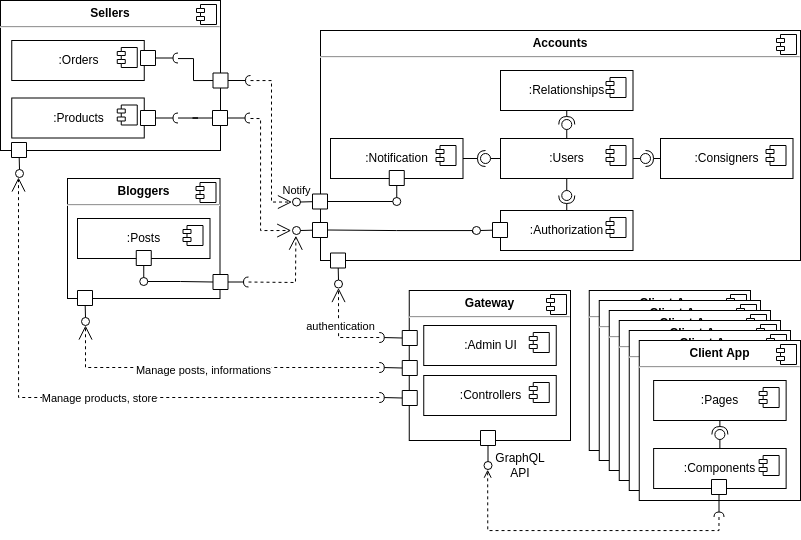
\includegraphics[width=\textwidth]{component}
		\caption{Sơ đồ thành phần hệ thống}
\justifying
Các ứng dụng phía máy khách giao tiếp với hệ thống máy chủ thông qua máy chủ trung tâm là gateway. Gateway sử dụng các dịch vụ quản lí của các máy chủ dịch vụ. Đối với máy chủ dịch vụ accounts, máy chủ gateway sử dụng chức năng authentication trả về cookie hoặc token cho ứng dụng máy khách.

Máy chủ dịch vụ sellers sử dụng chức năng gửi thông báo và chức năng lấy vai trò người dùng hiện tại của accounts. Nghĩa là khi một hành động mang theo \acrshort{headers} sellers căn cứ vào đó yêu cầu đến máy chủ dịch vụ accounts để biết được, ai là người đại diện cho truy vấn và ai là những người đóng góp cho người đại diện đó. Từ đó, sellers có thể căn cứ để trả về danh sách sản phẩm đúng với yêu cầu.
\end{figure}